% F049: native TikZ/PGFPlots, computed from the stated mathematical model.
\begin{center}
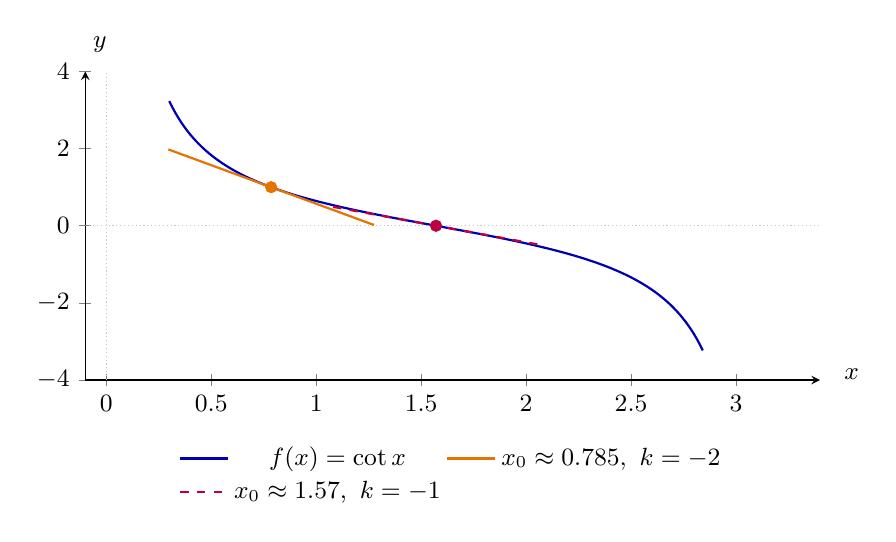
\begin{tikzpicture}[font=\small,>=stealth]
\begin{axis}[width=.90\linewidth,height=5.5cm,xmin=-0.1,xmax=3.4,ymin=-4,ymax=4,
axis lines=left,xlabel={$x$},ylabel={$y$},font=\small,
xlabel style={at={(axis description cs:1.02,.02)},anchor=west},
ylabel style={rotate=-90,at={(axis description cs:.02,1.03)},anchor=south},
legend style={at={(axis description cs:.5,-.18)},anchor=north,draw=none,fill=none,font=\small,legend columns=2},
unbounded coords=jump,clip=true,]
\addplot[gray!45,thin,densely dotted,forget plot] coordinates {(-0.1,0) (3.4,0)};
\addplot[gray!45,thin,densely dotted,forget plot] coordinates {(0,-4) (0,4)};
\addplot[blue!70!black,thick] coordinates {(0.3,3.2327281) (0.31411996,3.0780952) (0.32823992,2.9363447) (0.34235988,2.8058813) (0.35647984,2.6853621) (0.3705998,2.5736492) (0.38471976,2.4697712) (0.39883971,2.3728947) (0.41295967,2.2822999) (0.42707963,2.1973621) (0.44119959,2.1175368) (0.45531955,2.0423466) (0.46943951,1.9713718) (0.48355947,1.9042415) (0.49767943,1.8406269) (0.51179939,1.7802353) (0.52591935,1.7228057) (0.54003931,1.6681039) (0.55415927,1.6159198) (0.56827922,1.5660641) (0.58239918,1.5183657) (0.59651914,1.4726697) (0.6106391,1.4288356) (0.62475906,1.3867353) (0.63887902,1.3462522) (0.65299898,1.3072795) (0.66711894,1.2697196) (0.6812389,1.2334829) (0.69535886,1.1984869) (0.70947882,1.1646557) (0.72359878,1.1319193) (0.73771873,1.1002129) (0.75183869,1.0694766) (0.76595865,1.0396549) (0.78007861,1.0106961) (0.79419857,0.98255228) (0.80831853,0.95517874) (0.82243849,0.92853379) (0.83655845,0.90257853) (0.85067841,0.87727655) (0.86479837,0.85259378) (0.87891833,0.82849827) (0.89303829,0.80496003) (0.90715825,0.78195088) (0.9212782,0.75944432) (0.93539816,0.73741535) (0.94951812,0.71584043) (0.96363808,0.69469732) (0.97775804,0.67396499) (0.991878,0.65362357) (1.005998,0.6336542) (1.0201179,0.61403902) (1.0342379,0.59476108) (1.0483578,0.57580426) (1.0624778,0.55715322) (1.0765978,0.53879336) (1.0907177,0.52071077) (1.1048377,0.50289215) (1.1189576,0.48532482) (1.1330776,0.46799664) (1.1471976,0.45089598) (1.1613175,0.43401171) (1.1754375,0.41733313) (1.1895574,0.40084997) (1.2036774,0.38455237) (1.2177973,0.36843081) (1.2319173,0.35247613) (1.2460373,0.33667948) (1.2601572,0.32103233) (1.2742772,0.3055264) (1.2883971,0.29015369) (1.3025171,0.27490644) (1.3166371,0.2597771) (1.330757,0.24475836) (1.344877,0.22984308) (1.3589969,0.2150243) (1.3731169,0.20029524) (1.3872369,0.18564926) (1.4013568,0.17107987) (1.4154768,0.15658071) (1.4295967,0.14214552) (1.4437167,0.12776816) (1.4578367,0.11344259) (1.4719566,0.099162842) (1.4860766,0.084923029) (1.5001965,0.070717328) (1.5143165,0.05653997) (1.5284364,0.042385232) (1.5425564,0.028247428) (1.5566764,0.014120898) (1.5707963,-1.6081226e-16) (1.5849163,-0.014120898) (1.5990362,-0.028247428) (1.6131562,-0.042385232) (1.6272762,-0.05653997) (1.6413961,-0.070717328) (1.6555161,-0.084923029) (1.669636,-0.099162842) (1.683756,-0.11344259) (1.697876,-0.12776816) (1.7119959,-0.14214552) (1.7261159,-0.15658071) (1.7402358,-0.17107987) (1.7543558,-0.18564926) (1.7684758,-0.20029524) (1.7825957,-0.2150243) (1.7967157,-0.22984308) (1.8108356,-0.24475836) (1.8249556,-0.2597771) (1.8390756,-0.27490644) (1.8531955,-0.29015369) (1.8673155,-0.3055264) (1.8814354,-0.32103233) (1.8955554,-0.33667948) (1.9096753,-0.35247613) (1.9237953,-0.36843081) (1.9379153,-0.38455237) (1.9520352,-0.40084997) (1.9661552,-0.41733313) (1.9802751,-0.43401171) (1.9943951,-0.45089598) (2.0085151,-0.46799664) (2.022635,-0.48532482) (2.036755,-0.50289215) (2.0508749,-0.52071077) (2.0649949,-0.53879336) (2.0791149,-0.55715322) (2.0932348,-0.57580426) (2.1073548,-0.59476108) (2.1214747,-0.61403902) (2.1355947,-0.6336542) (2.1497147,-0.65362357) (2.1638346,-0.67396499) (2.1779546,-0.69469732) (2.1920745,-0.71584043) (2.2061945,-0.73741535) (2.2203144,-0.75944432) (2.2344344,-0.78195088) (2.2485544,-0.80496003) (2.2626743,-0.82849827) (2.2767943,-0.85259378) (2.2909142,-0.87727655) (2.3050342,-0.90257853) (2.3191542,-0.92853379) (2.3332741,-0.95517874) (2.3473941,-0.98255228) (2.361514,-1.0106961) (2.375634,-1.0396549) (2.389754,-1.0694766) (2.4038739,-1.1002129) (2.4179939,-1.1319193) (2.4321138,-1.1646557) (2.4462338,-1.1984869) (2.4603538,-1.2334829) (2.4744737,-1.2697196) (2.4885937,-1.3072795) (2.5027136,-1.3462522) (2.5168336,-1.3867353) (2.5309536,-1.4288356) (2.5450735,-1.4726697) (2.5591935,-1.5183657) (2.5733134,-1.5660641) (2.5874334,-1.6159198) (2.6015533,-1.6681039) (2.6156733,-1.7228057) (2.6297933,-1.7802353) (2.6439132,-1.8406269) (2.6580332,-1.9042415) (2.6721531,-1.9713718) (2.6862731,-2.0423466) (2.7003931,-2.1175368) (2.714513,-2.1973621) (2.728633,-2.2822999) (2.7427529,-2.3728947) (2.7568729,-2.4697712) (2.7709929,-2.5736492) (2.7851128,-2.6853621) (2.7992328,-2.8058813) (2.8133527,-2.9363447) (2.8274727,-3.0780952) (2.8415927,-3.2327281)};
\addlegendentry{$f(x)=\cot x$}
\addplot[orange!90!black,thick] coordinates {(0.29539816,1.98) (1.2753982,0.02)};
\addlegendentry{$x_0\approx0.785,\ k=-2$}
\addplot[only marks,mark=*,orange!90!black,forget plot] coordinates {(0.78539816,1)};
\addplot[purple,thick,dashed] coordinates {(1.0807963,0.49) (2.0607963,-0.49)};
\addlegendentry{$x_0\approx1.57,\ k=-1$}
\addplot[only marks,mark=*,purple,forget plot] coordinates {(1.5707963,6.123234e-17)};

\end{axis}
\end{tikzpicture}
\par\smallskip{\small $\sin x\ne0$；图中只画 $(0,\pi)$ 内的一段。}
\end{center}
